\documentclass[10pt]{article}

\usepackage{graphicx}
\usepackage[utf8]{inputenc}
\usepackage[swedish]{babel}
\usepackage[margin=2cm]{geometry}

\selectlanguage{swedish}
\graphicspath{ {images/} }

\title{Systemanatomi\\
    \large Projektgrupp 1}
    
\author{
    Joel Almqvist\\
    \texttt{joeal360@student.liu.se}
    \and
    Björn Detterfelt\\
    \texttt{bjode786@student.liu.se}
    \and
    Tim Håkansson\\
    \texttt{timha404@student.liu.se}
    \and
    David Kjellström\\
    \texttt{davkj168@student.liu.se}
    \and
    Axel Löjdquist\\
    \texttt{axelo225@student.liu.se}
    \and
    Joel Oskarsson\\
    \texttt{joeos014@student.liu.se}
    \and
    Lieth Wahid\\
    \texttt{liewa893@student.liu.se}
    \and
    Alexander Wilkens\\
    \texttt{alewi684@student.liu.se}
}

\begin{document}
	\maketitle
	
	\tableofcontents

	\pagebreak
	
	\section{Definitioner}
	\begin{itemize}
		\item IoT - Internet of Things, koncept som beskriver att många objekt är uppkopplade mot internet
		\item UI / UI-applikation - den applikation som håller i själva spelet och visar upp spelplanen i sitt grafiska gränssnitt
		\item Speldata - information om handlingar och status i spelet samt nödvändig teknisk data för att upprätthålla kommunikation
	\end{itemize}
	
	\section{Systemanatomi}	
		I figur \ref{fig:graf} visas en systemanatomi över det realtidsspel som ska utvecklas. Gröna noder representerar handlingar som sker på kontrollen i spelet. Röda noder representerar handlingar som sker på UI-applikationen, som hanterar och visar upp spelplanen. Beteckningen ``$= 1$`` betecknar logisk XOR.\\
	
		\begin{figure}[h]
			\centering
			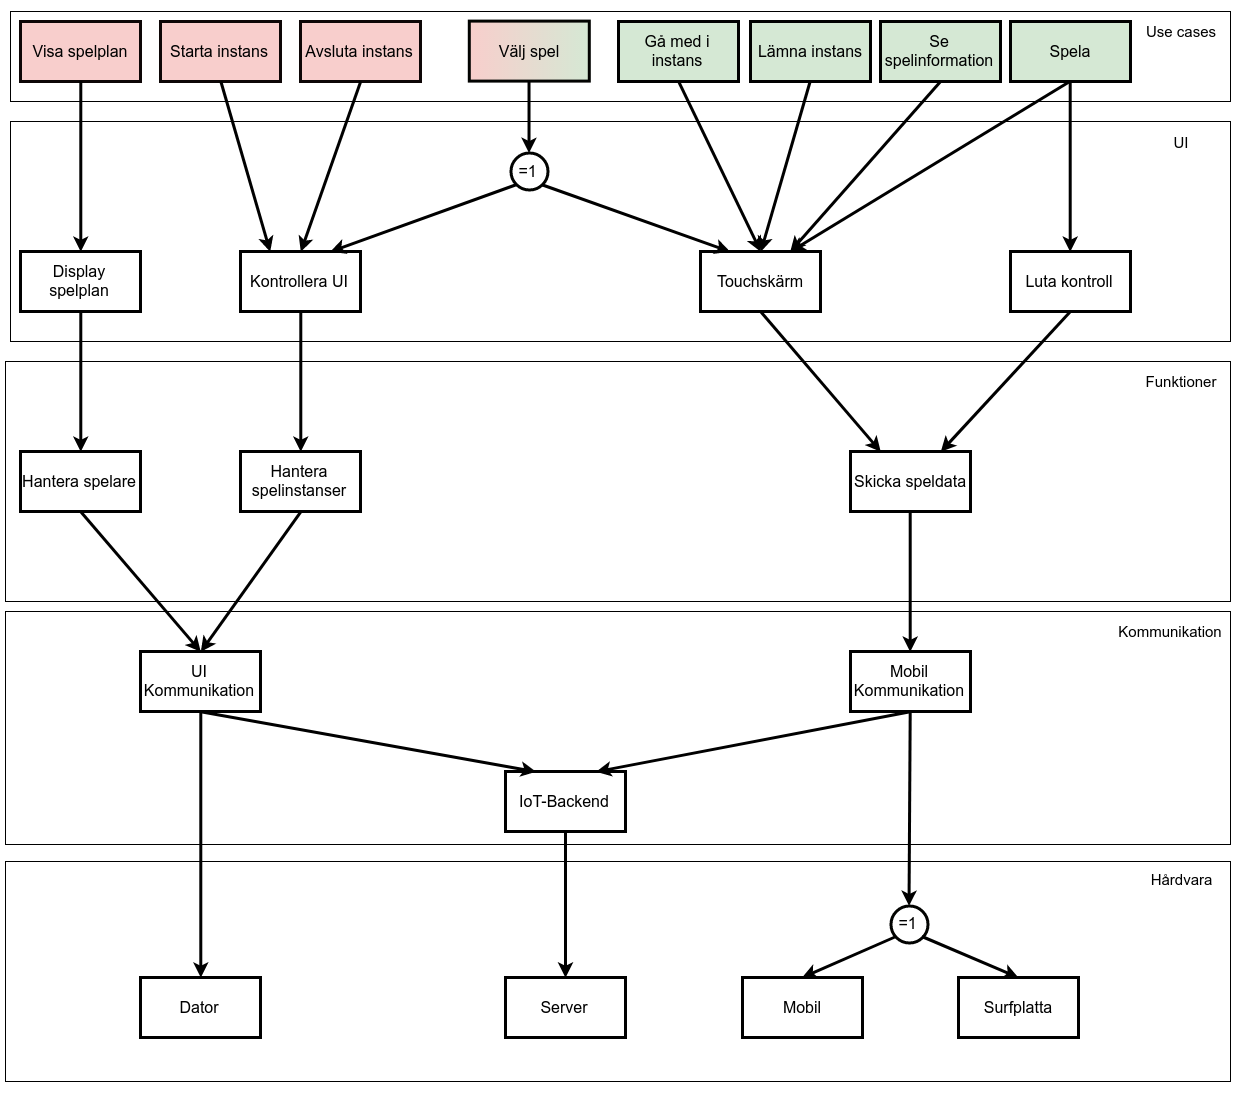
\includegraphics[scale=0.4]{systemanatomi_graf}
			\caption{Systemanatomi över realtidsspel på IoT-Backend}
			\label{fig:graf}
		\end{figure}	
	\pagebreak
	En spelinstans ska tolkas som den instans av spelet som startas från UI-applikationen och spelare kan gå med i för att spela spelet tillsammans. Spelarna lämnar denna instans genom att avsluta spelet på kontrollen, men instansen avslutas från UI-delen.\\
	
	IoT-Backend beskriver det system som Cybercom har skapat för kommunikation mellan enheter. Detta kommer ha en viktig roll i det slutgiltiga systemet och har därmed en central roll i systemanatomin.\\
	
\end{document}